\chapter{Theoretische Grundlagen}
\section{Äquivalenz}
\subsection{$\alpha$-Äquivalenz \slide{20}{166}}
gleicher Ausdruck / Funktion, nur andere Namen $\Rightarrow$ durch Umbenennung Transformation von $t_1$ zu $t_2$ möglich

\subsection{$\eta$-Äquivalenz \slide{20}{167}}
Zwei Funktionen sind gleich, falls Ergebnis gleich für alle Argumente

\subsection{Divergenz \slide{20}{182}}
Terme, die nicht zu einer Normalform auswerten, divergieren. Diese modellieren unendliche Ausführungen.

\subsection{Rekursionsoperator \slide{20}{184}}
$$Y= \lambda f.\; (\lambda x.\; f\; (x\; x))\; (\lambda x.\; f\; (x\; x))$$
mit 
$$f\; (Y\; f) \overset{\beta}{=} Y\; f$$ 
%\todo[inline]{$\overset{\beta}{=}$ Bedeutung: Gleich nach vollständiger $\beta$-Reduktion?}

\subsection{Auswertungsstrategien}
\begin{compactitem}
	\item Volle $\beta$-Reduktion \slide{20}{177}: Jeder Redex kann jederzeit reduziert werden
	\item Normalenreihenfolge \slide{20}{177}: Immer der linkeste äußerste Redex (der Parameter zur Verfügung hat) wird reduziert
	\item Call-By-Name \slide{20}{189}: Reduziere linkesten äußersten Redex, der nicht von einem $\lambda$ umgeben ist\\
	$\Rightarrow$ Reduziere Argumente erst, wenn benötigt
	\item Call-By-Value \slide{20}{190}: Reduziere linkesten äußersten Redex, der nicht von einem $\lambda$ umgeben ist und dessen Argument ein Wert (d.h. max. ausgewertet, darf auch ein Lambda-Ausdruck sein) ist\\
	$\Rightarrow$ werte Argumente vor Funktionsaufruf aus, dann setze max. ausgewertete Argumente ein
\end{compactitem}

\subsection{Church-Zahlen \slide{20}{179ff}}
\begin{compactitem}
	\item Zahlen:
		\begin{align*}
			c_0 &= \lambda s.\; \lambda z.\; z\\
			c_1 &= \lambda s.\; \lambda z.\; s\; z\\
			c_2 &= \lambda s.\; \lambda z.\; s\; (s\; z)\\
				& \vdots \\
			c_n &= \lambda s.\; \lambda z.\; s^n\; z
		\end{align*}
	\item Operationen
		\begin{compactitem}
			\item Nachfolgerfunktion $succ = \lambda n.\; \lambda s.\; \lambda z.\; s\; (n\; s\; z)$
			\item Addition $plus = \lambda m.\; \lambda n.\; \lambda s.\; \lambda z.\; m\; s\; (n\; s\; z)$
			\item Multiplikation $times = \lambda m.\; \lambda n.\; \lambda s.\; n\; (m\; s) \overset{\eta}{=} \lambda m.\; \lambda n.\; \lambda s.\; \lambda z.\; n\; (m\; s)\; z$
			\item Potenzieren $exp = \lambda m.\; \lambda n.\; n\; m \overset{\eta}{=} \lambda m.\; \lambda n.\; \lambda s. \; \lambda z.\; n\; m\; s\; z$
			\item Subtraktion $sub = \lambda m.\; \lambda n.\; n\; pred\; m$\exRef{ÜB 5, Nr. 4}
				\begin{compactitem}
					\item $pair = \lambda a.\; \lambda b.\; \lambda f.\; f\; a\; b$
					\item $fst = \lambda p.\; p (\lambda a.\; \lambda b.\; a)$
					\item $snd = \lambda p.\; p (\lambda a.\; \lambda b.\; b)$
					\item $next = \lambda p.\; pair\; (snd\; p)\; (succ\; (snd\; p))$
					\item $pred = \lambda n.\; fst\; (n\; next\; (pair\; c_0\; c_0))$
				\end{compactitem}
			\item Vegleichsoperation \enquote{lessEq $m \leq n$} $lessEq = \lambda m.\; \lambda n.\; isZero\; (sub\; m\; n)$\exRef{ÜB 6, Nr. 2}
			\item Vegleichsoperation \enquote{greaterEq $m \geq n$} $greaterEq = \lambda m.\; \lambda n.\; isZero\; (sub\; n\; m)$
			\item Vergleichsoperation \enquote{eq $m == n$} $eq = \lambda m.\; \lambda n.\; (\lambda a.\; a)\; (lessEq\; m\; n)\; (greaterEq\; m\; n)\; c_{false}$
			\item $isZero = \lambda n.\; n\; (\lambda p.\; c_{false})\; c_{true}$\exRef{SS 14}
		\end{compactitem}
	\item boolsche Werte
		\begin{compactitem}
			\item True $c_{true} = \lambda t.\; \lambda f.\; t$
			\item False $c_{false} = \lambda t.\; \lambda f.\; f$
		\end{compactitem}
\end{compactitem}

\subsection{Rekursionsoperator Y \slide{20}{184}}
$$Y=\lambda f. (\lambda x. f (x\; x))(\lambda x.f(x\; x))$$
\begin{compactitem}
	\item Rekursionsoperator Y ist nicht typisierbar \slide{21}{205}
\end{compactitem}

\section{Typinferenz}
Bei Let-Polymorphismus angepasste Regeln von VAR und ABS \slide{22}{211}\\
\iffalse
\noindent\makebox[\textwidth]{
\begin{tabular}{|c|c|c|}
	\hline 
	Regel & Constraint & Bsp. \\ 
	\hline 
	CONST\begin{LARGE}$\frac{c\;\in\; Const}{\Gamma\; \vdash\; c\; :\; \tau_c}$\end{LARGE}
	& \multlineTable{CONST\begin{LARGE}$\frac{c\;\in\; Const}{\Gamma\; \vdash\; c\; :\; \alpha_1}:$\end{LARGE}\\ $\alpha_1 = Typ(c)$ }
	& \multlineTable{CONST\begin{LARGE}$\frac{1\;\in\; Const}{\Gamma\; \vdash\; 1\; :\; \alpha_1}:$\end{LARGE}\\ $\alpha_1 = Typ(1)=Int$ } 
	\\[5ex]
	\hline 
	VAR\begin{LARGE}$\frac{\Gamma(x)\;=\;\tau}{\Gamma\; \vdash\; x\; :\; \tau}$\end{LARGE} 
	& \multlineTable{VAR\begin{LARGE}$\frac{(x:\;\alpha_1)(x)\;=\;\alpha_2}{(x\;:\;\alpha_1)\; \vdash\; x\;:\; \alpha_2}:$\end{LARGE}\\ $\alpha_1 = \alpha_2$ }
	& \\[5ex]
	\hline 
	ABS\begin{LARGE}$\frac{\Gamma,\;x\;:\;\tau_1\; \vdash\; t\;:\;\tau_2}{\Gamma\; \vdash\; \lambda x.t:\; \tau_1\; \rightarrow\; \tau_2}$\end{LARGE}
	& \multlineTable{ABS\begin{LARGE}$\frac{\Gamma,\;x\;:\;\alpha_2\; \vdash\; t\;:\;\alpha_3}{\Gamma\; \vdash\; \lambda x.t\;:\; \alpha_1}:$\end{LARGE}\\ $\alpha_1 = \alpha_2\; \rightarrow\; \alpha_3$ }  
	&  \\[5ex]
	\hline 
	APP\begin{LARGE}$\frac{\Gamma\; \vdash\; t_1\;:\;\tau_2\; \rightarrow\; \tau \qquad \Gamma\; \vdash\; t_2\; :\; \tau_2}{\Gamma\; \vdash\; t_1\; t_2:\; \tau}$\end{LARGE}
	& \multlineTable{APP\begin{LARGE}$\frac{\Gamma\; \vdash\; t_1\;:\;\alpha_2\; \qquad \Gamma\; \vdash\; t_2\; :\; \alpha_3}{\Gamma\; \vdash\; t_1\; t_2\;:\; \alpha_1}:$\end{LARGE} \\ $\alpha_2 = \alpha_3 \rightarrow \alpha_1$ }  
	& \\[5ex]
	\hline
	LET\begin{LARGE}$\frac{\Gamma\; \vdash\; t_1\;:\;\tau_1 \quad \Gamma,\; x\;:\; ta(\tau_1,\;\Gamma)\;\vdash\; t_2\; :\; \tau_2}{\Gamma\; \vdash\; let\; x = t_1\; in\; t_2\; :\; \tau_2}$\end{LARGE}
	& \multlineTable{LET\begin{LARGE}$\frac{\Gamma\; \vdash\; t_1\;:\;\alpha_2 \quad \Gamma,\; x\;:\; ta(\alpha_2,\;\Gamma)\;\vdash\; t_2\; :\; \alpha_3}{\Gamma\; \vdash\; let\; x = t_1\; in\; t_2\; :\; \alpha_1}:$\end{LARGE} \\ $\alpha_2 = \alpha_3$}  
	& \\[5ex]
	\hline
\end{tabular} 
}
\fi 

\noindent\makebox[\textwidth]{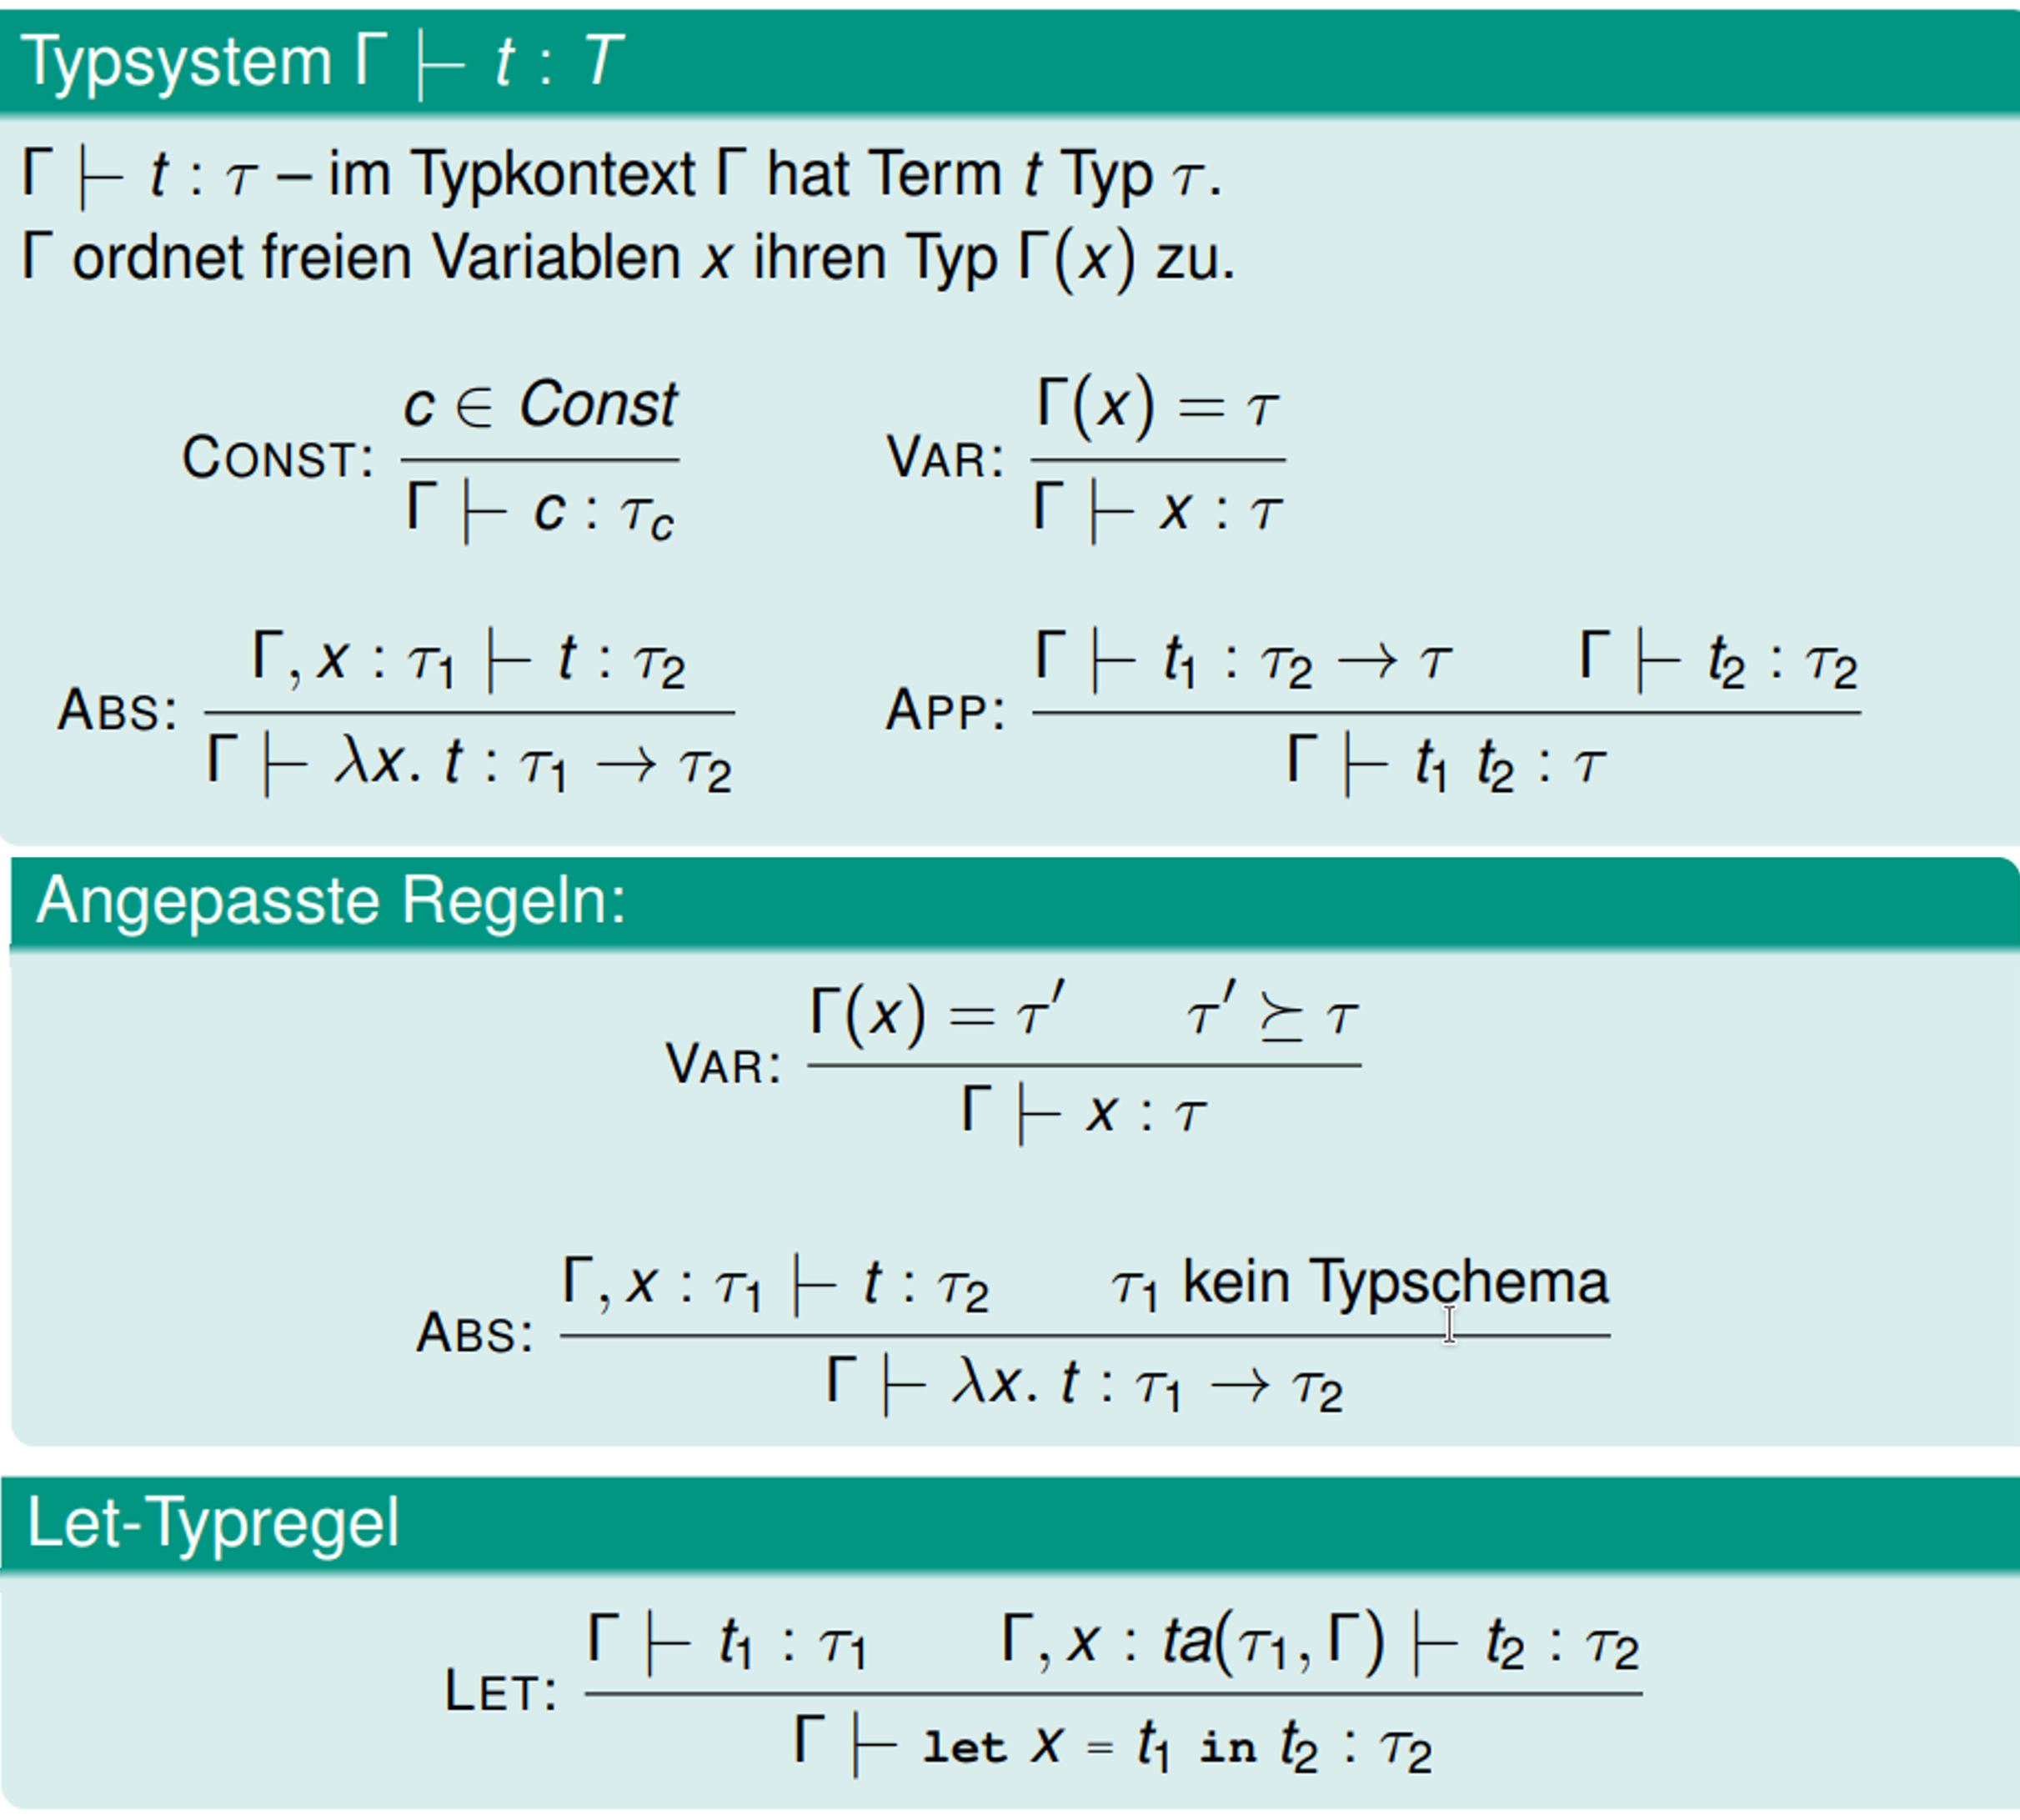
\includegraphics[scale=0.20]{imgs/TypinferenzCaptureCut.png}}